\documentclass[pdf,aspectratio=169]{beamer}
\usepackage[]{hyperref,graphicx,siunitx,booktabs,lmodern}
\usepackage{physics}
\usepackage{em-commands}
\mode<presentation>{\usetheme{EM}}

%Question Numbering
\newcounter{questionnumber}
\newcommand{\qnum}{%
	\stepcounter{questionnumber}%
	Q\arabic{questionnumber}
}
\resetcounteronoverlays{questionnumber}

\graphicspath{ {../Images/} }

\sisetup{per-mode=symbol}

\tikzstyle{plate}=[draw, very thick, minimum width=4cm, minimum height=1cm, fill=gray!40, anchor=south]

%preamble
\title{Magnetic Construction}
\date{October 31, 2018}
\author{Jed Rembold}

\begin{document}
\renewcommand{\theenumi}{\Alph{enumi}}

\begin{frame}{Announcements}
	\begin{itemize}
		\item Happy Spooky Day!
		\item Homework
			\begin{itemize}
				\item Homework 9 is posted and due on Monday (only 4 problems, but \emph{do not} delay starting them)
				\item Homework 10 is going to be super short (like 1 or 2 problems) and will be due a week from \emph{Friday}
				\item Homework 11 will be due after Thanksgiving
			\end{itemize}
		\item Test 2 will be on November 12, take-home portion will be due on the 14th
		\item Online schedule has been updated to reflect all the above
		\item Reminder: Grade reports posted to WISE Dropbox
		\item Read the rest of Chapter 5 by Friday
	\end{itemize}
\end{frame}

\begin{frame}{\qnum}
	\begin{columns}
		\column{0.75\textwidth}
		Ampere's Law will only be useful to us when there is sufficient symmetry to pull B out of the integral. So we need some methods to understand when we might have the needed symmetry.

		For the case of an infinitely long wire, can $\mf$ point radially (i.e., in the $\vu{s}$ direction)? \emph{Can you explain WHY?}
		\begin{enumerate}
			\item Yes
			\item \alert<2>{No}
		\end{enumerate}
		
		\column{0.25\textwidth}
		\begin{center}
			\begin{tikzpicture}
				\draw[very thick, Red, -latex] (0,0) -- +(0,6) node[above,math] {\cur};
				\draw[thick, -latex] (-.1,3) -- +(-1,0) node[midway,above] {$\mf$?};
			\end{tikzpicture}
		\end{center}
		
	\end{columns}
\end{frame}

\begin{frame}{\qnum}
	\begin{columns}
		\column{0.75\textwidth}
		Continuing to refine our arguments, for an infinitely long straight wire, can $\mf$ depend on $z$ or $\phi$? \emph{Why?}
		\begin{enumerate}
			\item Yes
			\item \alert<2>{No}
		\end{enumerate}
		
		\column{0.25\textwidth}
		\begin{center}
			\begin{tikzpicture}
				\draw[very thick, Red, -latex] (0,0) -- +(0,6) node[above,math] {\cur};
			\end{tikzpicture}
		\end{center}
	\end{columns}
\end{frame}

\begin{frame}{\qnum}
	\begin{columns}
		\column{0.75\textwidth}
		And finally, for an infinitely long straight wire, can $\mf$ have a component in the $\zhat$ direction? \emph{Why?}
		\begin{enumerate}
			\item Yes
			\item \alert<2>{No}
		\end{enumerate}
		
		\column{0.25\textwidth}
		\begin{center}
			\begin{tikzpicture}
				\draw[very thick, Red, -latex] (0,0) -- +(0,6) node[above,math] {\cur};
				\draw[thick, -latex] (-1,3) -- +(0,1) node[above] {$\mf$?};
			\end{tikzpicture}
		\end{center}
	\end{columns}
\end{frame}

\begin{frame}{\qnum}
	So our arguments got us a functional form of
	\[\mf(\pos) = B(s)\vu*{\phi}\]
	For the case of an infinitely long \emph{thick} wire of radius $a$, is this functional form still correct?
	\begin{enumerate}
		\item \alert<2>{Yes}
		\item Only inside the wire ($s < a$)
		\item Only outside the wire ($s > a$)
		\item No
	\end{enumerate}
\end{frame}

\begin{frame}{\qnum}
	\begin{columns}
		\column{0.7\textwidth}
		An infinite solenoid with surface current density $\scd$ is oriented along the $z$-axis. To use Ampere's Law, we need to argue what we know $\mf(\pos)$ should depend on and in what direction it should point.

		\vspace{1em}
		For this solenoid, $\mf(\pos)=$
		\begin{enumerate}
			\item $B(z) \zhat$
			\item $B(z) \vu*\phi$
			\item \alert<2>{$B(s) \zhat$}
			\item $B(s) \vu*\phi$
		\end{enumerate}
		
		\column{0.3\textwidth}
		\begin{center}
			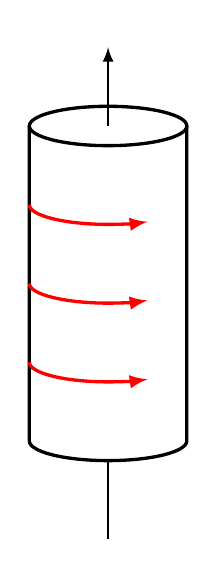
\begin{tikzpicture}
				\draw[very thick] (0,0) circle (1cm and .25cm);
				\draw[very thick] (-1,0) -- ++(0,-4) arc (180:360:1cm and .25cm)coordinate[midway] (m) --++(0,4);
				\draw[thick] (m) --+(0,-1);
				\draw[thick, -latex] (0,0) -- +(0,1) node[above] {$\zhat$};
				\foreach \y in {-1,-2,-3} \draw[Red, very thick ,-latex] (-1,\y) arc (180:300:1cm and .25cm);
				\node[Red] at (0,-1.75) {$\scd$};
			\end{tikzpicture}
		\end{center}
	\end{columns}
\end{frame}

\begin{frame}{\qnum}
	\begin{columns}
		\column{0.5\textwidth}
		\begin{center}
			\begin{tikzpicture}
				\foreach \y in {1,2,3} \draw[very thick, -latex, Red] (-.75,\y,4) -- +(0,0,-3);
				\pic[opacity=.5] at (-1,0) {box=teal/.5/4/4};
				\path[very thick, -latex]
				(0,0,0) edge node[at end, right]{$\yhat$} +(1,0,0)
				(0,0,0) edge node[at end, below]{$\xhat$} +(0,0,1)
				(0,0,0) edge node[at end, above]{$\zhat$} +(0,1,0);
			\end{tikzpicture}
		\end{center}
		\column{0.5\textwidth}
		What do you expect $\mf(\pos)$ to look like for the infinite current sheet to the left?
		\begin{enumerate}
			\item $B(y) \yhat$
			\item $B(z) \yhat$
			\item \alert<2>{$B(y) \zhat$}
			\item $B(z) \zhat$
		\end{enumerate}
	\end{columns}
\end{frame}

\begin{frame}{\qnum}
	\begin{columns}
		\column{0.5\textwidth}
		\begin{center}
			\begin{tikzpicture}
				\foreach \y in {1,2,3} \draw[very thick, -latex, Red] (-.75,\y,4) -- +(0,0,-3);
				\pic[opacity=.5] at (-1,0) {box=teal/.5/4/4};
				\draw[very thick, dashed] (1,0) rectangle +(1,3);
			\end{tikzpicture}
		\end{center}
		\column{0.5\textwidth}
		Suppose you drew the Amperian loop shown as a dashed line to the left. What would Ampere's Law tell you about the $z$-component of the magnetic field outside the current sheet?
		\begin{enumerate}
			\item \alert<2>{$B_z$ is constant outside the sheet}
			\item $B_z$ is 0 outside the sheet
			\item $B_z$ is not constant outside the sheet
			\item It tells you nothing about $B_z$.
		\end{enumerate}
	\end{columns}
\end{frame}

%\begin{frame}{\qnum}
	%What is necessary for
	%\[\laplacian\vA = -\mu_0 \vcd\]
	%\begin{enumerate}
		%\item $\curl\vA = 0$
		%\item $\div\vA = 0$
		%\item $\div\vA = \curl\vA$
		%\item $\vA \rightarrow 0$ at $\infty$
	%\end{enumerate}
%\end{frame}

%\begin{frame}{\qnum}
	%Assuming $\vcd$ goes to 0 at $\infty$, we can calculate $\vA$ in Cartesian using:
	%\[\vA(\pos) = \frac{\mu_0}{4\pi}\int \frac{\vcd(\pos_s)}{\srmag}d\tau_s\]
	%Can this integral also be done in spherical coordinates?
	%\begin{enumerate}
		%\item Yes, no problem
		%\item Yes, $r_s$ can be spherical but $\vcd$ needs to be in Cartesian components
		%\item Yes, $\vcd$ can be spherical, but $r_s$ needs to be in Cartesian components
		%\item No, this will not work due to cross terms in the spherical Laplacian
	%\end{enumerate}
	
%\end{frame}





\end{document}
